

\tikzset{every picture/.style={line width=0.75pt}} %set default line width to 0.75pt        

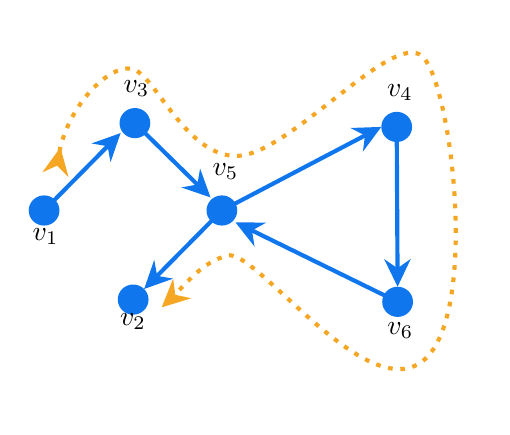
\begin{tikzpicture}[x=0.75pt,y=0.75pt,yscale=-1,xscale=1]
%uncomment if require: \path (0,186); %set diagram left start at 0, and has height of 186

%Shape: Ellipse [id:dp9872874664150777] 
\draw  [draw opacity=0][fill={rgb, 255:red, 15; green, 118; blue, 237 }  ,fill opacity=1 ] (25.01,84.75) .. controls (25.01,80.74) and (28.33,77.48) .. (32.42,77.48) .. controls (36.51,77.48) and (39.83,80.74) .. (39.83,84.75) .. controls (39.83,88.77) and (36.51,92.02) .. (32.42,92.02) .. controls (28.33,92.02) and (25.01,88.77) .. (25.01,84.75) -- cycle ;
%Shape: Ellipse [id:dp4278379475934897] 
\draw  [draw opacity=0][fill={rgb, 255:red, 15; green, 118; blue, 237 }  ,fill opacity=1 ] (67.92,127.67) .. controls (67.92,123.66) and (71.24,120.41) .. (75.33,120.41) .. controls (79.42,120.41) and (82.74,123.66) .. (82.74,127.67) .. controls (82.74,131.69) and (79.42,134.94) .. (75.33,134.94) .. controls (71.24,134.94) and (67.92,131.69) .. (67.92,127.67) -- cycle ;
%Shape: Ellipse [id:dp8609022262322172] 
\draw  [draw opacity=0][fill={rgb, 255:red, 15; green, 118; blue, 237 }  ,fill opacity=1 ] (68.76,42.66) .. controls (68.76,38.64) and (72.08,35.39) .. (76.17,35.39) .. controls (80.26,35.39) and (83.58,38.64) .. (83.58,42.66) .. controls (83.58,46.67) and (80.26,49.93) .. (76.17,49.93) .. controls (72.08,49.93) and (68.76,46.67) .. (68.76,42.66) -- cycle ;
%Shape: Ellipse [id:dp9159564206467596] 
\draw  [draw opacity=0][fill={rgb, 255:red, 15; green, 118; blue, 237 }  ,fill opacity=1 ] (110.67,84.75) .. controls (110.67,80.74) and (113.99,77.48) .. (118.08,77.48) .. controls (122.17,77.48) and (125.49,80.74) .. (125.49,84.75) .. controls (125.49,88.77) and (122.17,92.02) .. (118.08,92.02) .. controls (113.99,92.02) and (110.67,88.77) .. (110.67,84.75) -- cycle ;
%Shape: Ellipse [id:dp7639698933555006] 
\draw  [draw opacity=0][fill={rgb, 255:red, 15; green, 118; blue, 237 }  ,fill opacity=1 ] (195.33,128.75) .. controls (195.33,124.74) and (198.65,121.48) .. (202.74,121.48) .. controls (206.83,121.48) and (210.15,124.74) .. (210.15,128.75) .. controls (210.15,132.77) and (206.83,136.02) .. (202.74,136.02) .. controls (198.65,136.02) and (195.33,132.77) .. (195.33,128.75) -- cycle ;
%Shape: Ellipse [id:dp13383234090971663] 
\draw  [draw opacity=0][fill={rgb, 255:red, 15; green, 118; blue, 237 }  ,fill opacity=1 ] (194.9,44.48) .. controls (194.9,40.47) and (198.22,37.21) .. (202.31,37.21) .. controls (206.4,37.21) and (209.72,40.47) .. (209.72,44.48) .. controls (209.72,48.5) and (206.4,51.75) .. (202.31,51.75) .. controls (198.22,51.75) and (194.9,48.5) .. (194.9,44.48) -- cycle ;
%Straight Lines [id:da22310946546453647] 
\draw [color={rgb, 255:red, 15; green, 118; blue, 237 }  ,draw opacity=1 ][fill={rgb, 255:red, 0; green, 0; blue, 0 }  ,fill opacity=1 ][line width=1.5]    (32.42,84.75) -- (66.47,50.29) ;
\draw [shift={(69.28,47.45)}, rotate = 494.65] [fill={rgb, 255:red, 15; green, 118; blue, 237 }  ,fill opacity=1 ][line width=0.08]  [draw opacity=0] (13.4,-6.43) -- (0,0) -- (13.4,6.44) -- (8.9,0) -- cycle    ;
%Straight Lines [id:da332063115371956] 
\draw [color={rgb, 255:red, 15; green, 118; blue, 237 }  ,draw opacity=1 ][fill={rgb, 255:red, 0; green, 0; blue, 0 }  ,fill opacity=1 ][line width=1.5]    (109.75,75.66) -- (76.17,42.66) ;
\draw [shift={(112.61,78.46)}, rotate = 224.5] [fill={rgb, 255:red, 15; green, 118; blue, 237 }  ,fill opacity=1 ][line width=0.08]  [draw opacity=0] (13.4,-6.43) -- (0,0) -- (13.4,6.44) -- (8.9,0) -- cycle    ;
%Straight Lines [id:da6737055224421273] 
\draw [color={rgb, 255:red, 15; green, 118; blue, 237 }  ,draw opacity=1 ][fill={rgb, 255:red, 0; green, 0; blue, 0 }  ,fill opacity=1 ][line width=1.5]    (83.44,119.72) -- (118.08,84.75) ;
\draw [shift={(80.63,122.56)}, rotate = 314.73] [fill={rgb, 255:red, 15; green, 118; blue, 237 }  ,fill opacity=1 ][line width=0.08]  [draw opacity=0] (13.4,-6.43) -- (0,0) -- (13.4,6.44) -- (8.9,0) -- cycle    ;
%Straight Lines [id:da05298946125889348] 
\draw [color={rgb, 255:red, 15; green, 118; blue, 237 }  ,draw opacity=1 ][fill={rgb, 255:red, 0; green, 0; blue, 0 }  ,fill opacity=1 ][line width=1.5]    (202.31,44.48) -- (202.72,117.48) ;
\draw [shift={(202.74,121.48)}, rotate = 269.68] [fill={rgb, 255:red, 15; green, 118; blue, 237 }  ,fill opacity=1 ][line width=0.08]  [draw opacity=0] (13.4,-6.43) -- (0,0) -- (13.4,6.44) -- (8.9,0) -- cycle    ;
%Straight Lines [id:da10615226384080634] 
\draw [color={rgb, 255:red, 15; green, 118; blue, 237 }  ,draw opacity=1 ][fill={rgb, 255:red, 0; green, 0; blue, 0 }  ,fill opacity=1 ][line width=1.5]    (202.74,128.75) -- (128.2,92.22) ;
\draw [shift={(124.61,90.46)}, rotate = 386.11] [fill={rgb, 255:red, 15; green, 118; blue, 237 }  ,fill opacity=1 ][line width=0.08]  [draw opacity=0] (13.4,-6.43) -- (0,0) -- (13.4,6.44) -- (8.9,0) -- cycle    ;
%Straight Lines [id:da39588218363678185] 
\draw [color={rgb, 255:red, 15; green, 118; blue, 237 }  ,draw opacity=1 ][fill={rgb, 255:red, 0; green, 0; blue, 0 }  ,fill opacity=1 ][line width=1.5]    (118.08,84.75) -- (191.36,46.34) ;
\draw [shift={(194.9,44.48)}, rotate = 512.3399999999999] [fill={rgb, 255:red, 15; green, 118; blue, 237 }  ,fill opacity=1 ][line width=0.08]  [draw opacity=0] (13.4,-6.43) -- (0,0) -- (13.4,6.44) -- (8.9,0) -- cycle    ;
%Curve Lines [id:da6278709018521982] 
\draw [color={rgb, 255:red, 245; green, 166; blue, 35 }  ,draw opacity=1 ][line width=1.5]  [dash pattern={on 1.69pt off 2.76pt}]  (39.83,56.33) .. controls (44.44,33.79) and (63.66,14.42) .. (74.61,16.46) .. controls (85.74,18.53) and (100.46,59.15) .. (125.61,58.46) .. controls (150.76,57.78) and (200.38,-2.33) .. (214.61,10.46) .. controls (228.83,23.25) and (242.41,136.35) .. (214.61,157.46) .. controls (186.8,178.57) and (134.11,102.52) .. (120.61,106.46) .. controls (108.12,110.1) and (102.9,118.08) .. (91.9,128.75) ;
\draw [shift={(89.1,131.4)}, rotate = 317.28999999999996] [fill={rgb, 255:red, 245; green, 166; blue, 35 }  ,fill opacity=1 ][line width=0.08]  [draw opacity=0] (13.4,-6.43) -- (0,0) -- (13.4,6.44) -- (8.9,0) -- cycle    ;
\draw [shift={(40.27,54.37)}, rotate = 460.31] [fill={rgb, 255:red, 245; green, 166; blue, 35 }  ,fill opacity=1 ][line width=0.08]  [draw opacity=0] (13.4,-6.43) -- (0,0) -- (13.4,6.44) -- (8.9,0) -- cycle    ;

% Text Node
\draw (25.43,91.78) node [anchor=north west][inner sep=0.75pt]    {$v_{1}$};
% Text Node
\draw (67.5,133.05) node [anchor=north west][inner sep=0.75pt]    {$v_{2}$};
% Text Node
\draw (69.18,20.8) node [anchor=north west][inner sep=0.75pt]    {$v_{3}$};
% Text Node
\draw (196.16,22.62) node [anchor=north west][inner sep=0.75pt]    {$v_{4}$};
% Text Node
\draw (112.09,60.42) node [anchor=north west][inner sep=0.75pt]    {$v_{5}$};
% Text Node
\draw (196.33,137.15) node [anchor=north west][inner sep=0.75pt]    {$v_{6}$};


\end{tikzpicture}